\documentclass[a4paper,12pt]{article}


\usepackage[utf8]{inputenc} % allow utf-8 input
\usepackage[T1]{fontenc}    % use 8-bit T1 fonts
\usepackage{hyperref}       % hyperlinks
\usepackage{url}            % simple URL typesetting
\usepackage{booktabs}       % professional-quality tables
\usepackage{amsfonts}       % blackboard math symbols
\usepackage{nicefrac}       % compact symbols for 1/2, etc.
\usepackage{microtype}      % microtypography
\usepackage{xcolor}         % colors

\usepackage{adjustbox}
% \usepackage[margin=2cm]{geometry}
\usepackage{amsmath}
\usepackage{amssymb}
\usepackage{amsthm}
\usepackage{tcolorbox}
\usepackage{amsfonts}
\usepackage{stmaryrd}
\usepackage{xcolor}
\usepackage{algpseudocode}
\usepackage{algorithm}
\usepackage{mathtools}
\usepackage{dsfont}
\usepackage{tikz}
\usepackage{tikz-cd}
\usepackage{bussproofs}
\usepackage{listings, lstautogobble}
\usepackage{caption}
\usepackage{subcaption}
\usepackage{graphicx}
\usepackage{svg}
\usepackage{float}
\usepackage{appendix}
\usepackage{natbib}
\bibliographystyle{plainnat}
%\usepackage[french]{babel}
\usepackage{multicol}
\usepackage{multirow}
\usepackage{tabularx}
\usepackage[percent]{overpic}
\usepackage{todonotes}
\usepackage{hyperref}
\hypersetup{
    colorlinks,
    linkcolor={red!50!black},
    citecolor={blue!50!black},
    urlcolor={blue!80!black}
}
\usetikzlibrary{bayesnet}



\newcommand{\dd}{\text{d}}
\renewcommand{\vec}{\overrightarrow}
\renewcommand{\Im}{\mathfrak{Im}\ }
\newcommand{\Ker}{\text{Ker}\ }
\newcommand{\bijective}{%
  \hookrightarrow\mathrel{\mspace{-15mu}}\rightarrow
}
\newcommand{\surjective}{\twoheadrightarrow}
\newcommand{\injective}{\hookrightarrow}
\newcommand{\implication}{\Longrightarrow}
\newcommand{\reciprocal}{\Longleftarrow}
\newcommand{\equivalent}{\Longleftrightarrow}
\newcommand{\NN}{\ensuremath{\mathbb{N}}}
\newcommand{\RR}{\ensuremath{\mathbb{R}}}
\newcommand{\QQ}{\ensuremath{\mathbb{Q}}}
\newcommand{\ZZ}{\ensuremath{\mathbb{Z}}}
\newcommand{\CC}{\ensuremath{\mathbb{C}}}
\newcommand{\EE}{\ensuremath{\mathbb{E}}}
\newcommand{\PP}{\ensuremath{\mathbb{P}}}
\newcommand{\II}{\ensuremath{\mathds{1}}}
\newcommand{\cR}{\ensuremath{\mathcal{R}}}
\newcommand{\cY}{\ensuremath{\mathcal{Y}}}
\newcommand{\cZ}{\ensuremath{\mathcal{Z}}}
\newcommand{\cX}{\ensuremath{\mathcal{X}}}
\newcommand{\cN}{\ensuremath{\mathcal{N}}}
\newcommand{\cT}{\ensuremath{\mathcal{T}}}

\renewcommand{\epsilon}{\varepsilon}
\renewcommand{\phi}{\varphi}
\newcommand{\floor}[1]{\left\lfloor #1 \right\rfloor}
\newcommand{\ceil}[1]{\left\lceil #1 \right\rceil}
\newcommand{\comb}[2]{\displaystyle{#2 \choose #1}}
\newcommand{\parts}{\mathcal{P}}
\newcommand{\permut}{\mathfrak{S}}
\newcommand{\id}{\text{Id}}
\newcommand{\indic}{\mathds{1}}
\newcommand{\indickronecker}[1]{\indic\left\{#1\right\}}
\renewcommand{\leq}{\leqslant}
\renewcommand{\geq}{\geqslant}
\newcommand{\mat}[2]{\mathcal{M}_{#1}(#2)}

\newcommand{\set}[1]{\ensuremath{\left\{ #1 \right\}}}
\newcommand{\Tau}{\mathcal{T}}

\newcommand{\norm}[1]{\ensuremath{\left|\left|#1\right|\right|}}
\newcommand{\card}[1]{\ensuremath{\left|#1\right|}}

\DeclareMathOperator{\mut}{mut}
\DeclareMathOperator{\stab}{Stab}
\DeclareMathOperator{\sg}{sg}
\DeclareMathOperator*{\argmax}{argmax}
\DeclareMathOperator*{\argmin}{argmin}
\renewcommand{\time}{\textsc{Time}}
\newcommand{\len}{\textsc{Length}}
\newcommand{\call}[1]{\textsc{#1}}
\newcommand{\bbrack}[1]{\left\llbracket#1\right\rrbracket}
\newtheorem{proposition}{Proposition}
\newtheorem{lemma}{Lemma}
\newtheorem{thm}{Theorem}
\newtheorem{definition}{Definition}
\newtheorem{example}{Example}
\DeclareMathOperator{\ucb}{UCB}
\DeclareMathOperator{\lcb}{LCB}

\newcommand{\tm}[1]{\todo[inline,color=orange!40]{{\textbf{TM:}~}#1}}
\newcommand{\TM}[1]{{\color{orange!40!red}#1}}
\newcommand{\tr}[1]{\todo[inline,color=blue!40]{{\textbf{TR:}~}#1}}
\newcommand{\TR}[1]{{\color{lightblue!40!blue}#1}}
\newcommand{\ar}[1]{\todo[inline,color=green!40]{{\textbf{AR:}~}#1}}
\newcommand{\AR}[1]{{\color{lime!40!green}#1}}

\title{Clustering Multivariate Ordinal Data}


\author{Thomas \textsc{Michel}, Théo \textsc{Rudkiewicz} and Ali \textsc{Ramlaoui}}



\begin{document}
\maketitle

% \tableofcontents

% %\section{TODOs}
%\begin{itemize}
%    \item For the experiments:
%    \begin{itemize}
%        \item Test the robustness of the algorithm when facing outliers or skewed distributions.
%        \item Use noisy ordinal data (add discrete noise on a few features).
%        \item Test scalability of the algorithm (number of variables and data points).
%    \end{itemize}
%\end{itemize}

\section{Introduction}
The exploration of hidden structures within datasets is a crucial task for data scientists, and clustering serves as a valuable tool for this. Mixture models have emerged as a standard approach for clustering due to their capacity to provide a well-defined mathematical framework for parameter estimation and model selection. These models, instrumental in determining the number of clusters, not only encapsulate classical geometric methods but also find successful application in diverse practical scenarios.

In the realm of model-based clustering, the classification of data hinges on the availability of a suitable probability distribution tailored to the nature of the data at hand—be it numerical, rankings, functional, or categorical. Notably, ordinal data, where categories possess a specific order, represent a common occurrence, especially in fields like marketing where product evaluations are solicited through ordinal scales. Despite their prevalence, ordinal data have received comparatively less attention in the context of model-based clustering. Often, practitioners resort to transforming ordinal data into quantitative or nominal formats to align with readily applicable distributions, neglecting valuable order information.

This paper delves into the less-explored domain of model-based clustering for ordinal data, specifically focusing on ordinal data derived from sample surveys. Ordinal data find widespread application in fields such as social sciences, psychology, marketing, healthcare, and more. They enable researchers to capture nuanced information, such as preferences, attitudes, or severity levels, in cases where continuous measures are neither significant nor possible. For example, when assessing tumor severity, the precise size may not be as crucial as the current state of development of the disease as assessed by specialists. The use of ordinal data enriches the comprehension of subjective opinions, behaviors, and hierarchical relationships across diverse research contexts.

Multiple approaches have been proposed to model ordinal data. The first primary approach involves modeling a function of the cumulative probabilities of the ordinal categories as a linear function of some covariates. A comprehensive review of these models can be found in \cite{agresti2010analysis}. The second main approach involves modeling the ordinal categories as a function of a latent continuous variable, which is then linked to the ordinal categories through a link function. We assume that the ordinal observations are generated by a form of discretization of the latent continuous variable. An illustrative example of this approach is the ordered probit model, a generalization of the probit model for ordinal data.

A final approach that will particularly interest us in this paper is the use of a probabilistic model that directly captures the data-generating process for ordinal data, ensuring it exhibits desired properties. Two main models have been proposed in this category. The first and most studied one is the CUB model and its extensions \citep{d2005mixture}, which suggests modeling the data-generating process as a mixture of uniform and binomial distributions. Later, an additional Dirac distribution was introduced in the mixture, removing the dependence on the distance between categories imposed by the binomial distribution with the nonlinear CUB model \citep{manisera2014modeling}.
Another notable model in this category is the Binary Ordinal Search model, proposed by \cite{biernacki2016model}. This model posits that the observed data is the outcome of a stochastic process involving a binary search algorithm with corrupted comparisons. Parameterized with a position parameter (modal category) and a precision parameter, this model exhibits desirable properties similar to those of the CUB model. These properties include a unique mode, a probability distribution decrease on either side of the mode, and the flexibility to accommodate uniform or Dirac distributions.

In the context of clustering, a common approach is to use a mixture model for clustering the data. The mixture model is a probabilistic model that assumes the data is generated by a convex combination of several probability distributions. The clustering process then assigns each data point to the most likely distribution component given the data. In the case of the BOS model, maximum likelihood estimation using an EM algorithm can be employed, leveraging the latent variable interpretation of the binary search algorithm. While combinatorial complexity limits straightforward estimation for models based on latent Gaussian variables, the proposed approach remains tractable for ordinal data with up to eight categories—a common scenario for most ordinal variables. By contrast, the CUB model cannot be used for clustering in this way, as two CUB distributions cannot be distinguished from one another due to the uniform distribution component.


In this paper, we replicate and extend the findings of \cite{biernacki2016model}. We re-implemented their suggested probabilistic model, parameter estimation method, and model-based clustering algorithm in Python. Taking inspiration from their approach, we propose an alternative probabilistic model with similar properties. The aim is to address computational limitations, enabling the clustering of more extensive datasets with more categories than what the previous method allows. We also present an analysis of this new method to justify the decreased computational cost of estimating parameters for this model. Additionally, we test \cite{biernacki2016model}'s approach on real-world datasets and compare it to the proposed approach, along with baseline models. This is conducted on different datasets of multiple natures to check whether the proposed methods are successful in these practical settings and to identify their advantages. The ultimate goal is to assess whether the gains are significant against methods not adapted for ordinal datasets, deciding whether these approaches are interesting to use as a default method of choice for this type of variable.




\input{bos_model_appendix.tex}

% \subsection{Alternative model "Globally Ordered Data" (GOD)}


% \tm {Laisser présentation du modèle, graphical model, estimation des paramètres. Tous les lemmes et théorèmes vont en annexe.}

In the article under study, the authors motivated the use of binary search with the following sentence: "In order to minimize the number of potentially wrong comparisons, it
is necessary to minimize the number of comparisons performed during the search process.". However, we believe that minimizing the number of incorrect comparisons may not be an adequate intuition, and it is more crucial to minimize the probability of making a wrong guess. Motivated by this perspective, we have developed an alternative model where the data is compared with each category with some noise. We will refer to this model as the Globally Ordered Data (GOD) model.

We still consider a search for the parameter $\mu$ among the ordered categories. However, instead of conducting a binary search, we compare each category to the parameter $\mu$ and with probability $\pi$ we get the correct answer. After making all these comparisons, we then select the category that corresponds to the minimum number of comparison error. This approach display similar properties to the BOS model such as a unique mode, probability distribution decrease on either side of the mode, and the flexibility to accommodate uniform or Dirac distribution.

\subsubsection{Probabilistic model}

\begin{figure}[htbp]
    \centering
    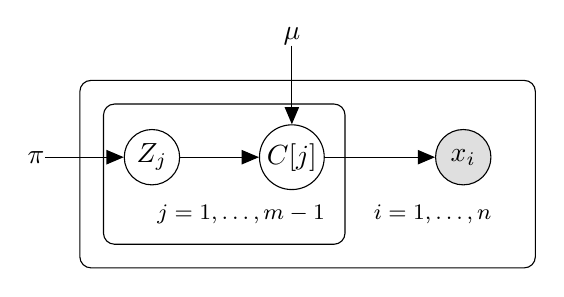
\begin{tikzpicture}
     \node[obs]                               (xj) {$x_i$};
     \node[latent, left=1.4cm of xj]               (cj) {$C[j]$};
     \node[latent, left=of cj]               (zj) {$Z_j$};
     \node[const, left=of zj]    (pi) {$\pi$};
     \node[const, above=of cj]  (mu) {$\mu$};
    
     \edge{zj}{cj};
     \edge{cj}{xj};
     \edge {mu} {cj};
     \edge {pi} {zj};
    
     \plate[inner sep=.55cm] {}{(xj)(cj)(zj)}{$i=1, \ldots, n$};
     \plate[inner sep=.25cm] {}{(cj)(zj)}{$j=1, \ldots, m - 1$};
    \end{tikzpicture}
    \caption{Graphical model of the GOD model.}
    \label{fig:god_graphical_model}
\end{figure}
    
The GOD model for $m$ categories is characterized by two parameters $\mu \in \bbrack{1, m}, \pi \in ]\frac{1}{2}, 1]$. The observed data is only the selected category $x$. The latent variables are the vector $Z = (Z_1,...,Z_{m-1}) \in \set{0, 1}^{m - 1}$ and $C \in \set{0, 1}^{m-1}$.
$(Z_j)_{j\in\bbrack{1,m-1}}$ is a vector of independent Bernoulli variables, with parameter $\pi$. For $j \in \bbrack{1, m-1}$, $Z_j$ indicates whether the comparison with the category $j$ is correct $(Z_j=1)$ or not $(Z_j=0)$. $C$ is the vector containing the $m$ results of the comparisons depending on both $Z$ and the parameter $\mu$. It is defined as follows:
\[
\forall j \in \bbrack{1, m-1}, C[j] = \begin{cases}
    (\mu < j) & \text{if}\  Z_j = 1\\
    (\mu \not< j) & \text{if}\  Z_j = 0
\end{cases} \]

The GOD model will generate $x \in \bbrack{1, m}$ such that $x \sim \mathcal{U}(\argmin_{k \in \bbrack{1, m}} \norm{c - E_k}_1)$. We can interpret this as a probability maximization as stated in Theorem~\ref{thm:projection}. The graphical model associated with this probabilistic model is depicted on Figure \ref{fig:god_graphical_model}.


\begin{definition}[Heaviside vector]
    For $k \in \bbrack{1, m}$, we define:
    \[E_k := (1)^{k-1} (0)^{m - k} = (\underset{k-1}{\underbrace{1, \dots, 1}}, \underset{m - k}{\underbrace{0, \dots, 0}} ). \]
\end{definition}


\begin{thm}
    \label{thm:projection}
    If we suppose that the prior distribution of $\mu$ is uniform over $\bbrack{1, m}$ and $\pi > \frac{1}{2}$, then \(\forall c \in \set{0, 1}^{m-1}\),
    \[\argmax_{k \in \bbrack{1, m}} \Pr(\mu = k | C = c) = \argmin_{k \in \bbrack{1, m}} \norm{c - E_k}_1.\]
\end{thm}

The proof can be found in appendix~\ref{thm:projection_appendix}.

\subsubsection{Parameter estimation}

We want to estimate $\pi$ and $\mu$ from a sample $X = (x^1, \dots, x^n) \in \bbrack{1, m}^n$ of $n$ observations of $x$ generated by the GOD model. We aim at maximizing the likelihood of the sample : $\Pr(X | \pi, \mu)$. 

We define for $x \in \bbrack{1, m}$, 
\[ \mathcal{C}_x := \set{c \in \set{0, 1}^{m-1} | x \in \argmin_{k \in \bbrack{1, m}} \norm{c - E_k}_1 } .\]

\begin{lemma}
    \label{lemma:p_x_c_knowing_pi_mu}
    \[\Pr(x, c | \pi, \mu) = \indic{}_{\mathcal{C}_x}(c) \frac{\pi^{m - 1 - \norm{c - E_{\mu}}_1} (1 - \pi)^{\norm{c - E_{\mu}}_1}}{\card{\argmin_{k \in \bbrack{1, m}} \norm{c - E_k}_1}} .\]
\end{lemma}

Proof in appendix~\ref{lemma:p_x_c_knowing_pi_mu_appendix}.


\begin{definition}
    We define for $x \in \bbrack{1, m}, \mu \in \bbrack{1, m}, d \in \bbrack{0, m-1}$:
    \[ u(\mu, x, d) := \sum_{c \in \mathcal{C}_x / \norm{c - E_{\mu}}_1 = d}  \card{\argmin_{k \in \bbrack{1, m}} \norm{c - E_k}_1}^{-1} .\]
\end{definition}

For a given $m$, $u$ can be fully computed in $\mathcal O(m^2 2^m)$ time. We believe that it might be possible to compute it in polynomial time, but we did not have time to find how. Although still costly, it only needs to be computed once for a given $m$ and can be stored in $\mathcal O(m^3)$ space.
% copilot :
% Indeed, for a given $x$ and $\mu$, we have $\card{\mathcal{C}_x} = \binom{m}{\mu}$ and $\card% {\argmin_{k \in \bbrack{1, m}} \norm{c - E_k}_1} = \binom{m}{\mu - d} \binom{m - \mu + d}{d}$. Therefore, we have:

\begin{definition}[weighted likelihood]
    For the AECM algorithm, we define the weighted likelihood with weights $w \in \RR_+^n$:
    \[ \Pr((X, W') | \pi, \mu) = \prod_{i=1}^{n} \Pr(x^i | \pi, \mu)^{w'_i} \]

    As  $X \in \bbrack{1, m}^n$, without loss of generality, we can assume that we have exactly $m$ weights: $W = (\sum_{i / x^i = 1} W'[i], \dots, \sum_{i / x^i = m} W'[i])$. Hence with $W \in \RR_+^m$:
    \[ \Pr((X, W') | \pi, \mu) = \Pr(W | \pi, \mu) = \prod_{i=1}^{m} \Pr(i | \pi, \mu)^{w_i} \]

    And again, without loss of generality, we can assume that every sample is weighted with weight $w'_i = 1$.

    Hence we now consider data as a vector $W \in \RR_+^m$.
\end{definition}

\begin{thm}[Data likelihood]
    \label{thm:p_xs_knowing_pi_mu}
    \begin{align}
        \Pr(W | \pi, \mu) 
        &= \pi^{(m-1)\sum_{i=1}^{m} w_i} \prod_{i=1}^{m} \left[\sum_{d = 0}^{m-1} \left(\frac{1 - \pi}{\pi}\right)^d u(x^i, \mu, d) \right]^{w_i}\\
        L_W(\pi, \mu) 
        &= (m-1)\left(\sum_{i=1}^{m} w_i\right) \log\pi + \sum_{i=1}^{m} w_i \log\left[ \sum_{d = 0}^{m-1} \left(\frac{1 - \pi}{\pi}\right)^d u(x^i, \mu, d) \right]
    \end{align}
\end{thm}
\begin{proof}
    We just use the fact that the random variables $(x^i)_{i=1}^n$ are independent and Theorem~\ref{thm:p_x_knowing_pi_mu} from Appendix~\ref{appendix:god}.
\end{proof}

Similarly to the BOS model, we estimate $\hat{\pi}$ for each fixed $\mu$. Then we keep the couple $(\hat{\pi}, \mu)$ that maximizes the log-likelihood.
To estimate $\pi$ for a fixed $\mu$, we considered different possibilities. The first option is to use a simple grid search. This is feasible as evaluating $L_X$ is not too costly and can be done in $\mathcal O(nm)$ time. Then, we considered using the EM algorithm, similar to the approach taken for the BOS model. We derived the update rules and implemented it. Unfortunately, there was an issue with our EM implementation for this model that we did not succeed in fixing.

\begin{figure}
    \centering
    \includegraphics[width=0.5\textwidth]{Attachments/log_likelihoods.png}
    \caption{Log-likelihoods for each possible $\mu$ for $n = 100$ samples with the true parameters being $m = 5$, $\mu=2$ and $\pi = 0.8$ }
    \label{fig:log_likelihoods}
\end{figure}

We can examine the log-likelihood functions in Figure~\ref{fig:log_likelihoods} to understand how to optimize them. As observed, each of the functions $\pi \mapsto L_X(\pi, \mu)$ is concave on the interval $[0.5, 1]$.

\begin{thm}
    \label{thm:log_likelihood_concave}
    $\forall \mu \in \bbrack{1, m}$, 
    \[ \pi \mapsto L_W(\pi, \mu) \]
    is concave on $[0.5, 1]$.
\end{thm}

For the proof, see appendix~\ref{thm:log_likelihood_concave_appendix}.

As the log-likelihood is concave, we can employ the trichotomy method to find the maximum with a few evaluations of $L_W$. For a precision $\epsilon$, the trichotomy method requires $k \geq \frac{\lg_2 \epsilon + 1}{1 - \lg_2 3} = \mathcal O(\ln \epsilon)$ steps and therefore $\mathcal O(\ln \epsilon)$ evaluation of $L_X$.

\paragraph{Complexity}

The pre-computational cost of computing $u$ is $\mathcal O(m^2 2^m)$.

The evaluation of $L_W$ is done in $\mathcal O(n + m^2)$. We run the trichotomy algorithm $m$ times, and therefore, we evaluate $L_W$ $\mathcal O(m \ln \epsilon)$ times. The total cost is thus $\mathcal O(n + m^2 \ln \epsilon)$ for $m$ being the number of categories, $n$ the number of observations and $\epsilon$ being the precision on $\pi$.

% %EM on the probabilistic model + algorithm
\section{Experiments}
In this section, we try to evaluate the performance of the two models on different datasets. We first present the experimental setup and the datasets used for the experiments. We then present the results obtained for the estimation algorithms on synthetic data and on real-life datasets. We finally try to discuss the results obtained and the relevance of the models. 

The goal of these experiments is to compare the two models but also to individually test their ability to cluster ordinal datasets and to check whether they are able to generalize to real-life datasets.

All of the experiments and table are reproducible using the provided code and datasets and the fixed seeds.

\subsection{Synthetic data}
\paragraph{Experimental setup.}
In this section, we propose to test the AECM algorithm for the BOS and the GOD model on synthetic data in order to check the ability of our proposed estimation methods to correctly estimate the parameters of the dataand to cluster the datasets. 

\paragraph{Runtimes.}
The runtimes of the AECM algorithm implementation with exponential complexity from \citet{biernacki2016model} 
are compared to our implementation of the AECM algorithm with polynomial complexity. Figure~\ref{fig:runtime_epsilon}  compare both complexities for multiple runtimes for both univariate and multivariate AECM runs. The runtimes are reported with different number of categories in the dataset $m$. While the original implementation struggles to go further than $m=6$, our implementation can easily reach higher number of categories. The implementation ordinalClust \cite{selosse2021ordinalclust} is used for fair comparison and it is allowed to converge with a predefined $\epsilon$ parameter (internal to the authors package that we cannot modify). 
The worst case complexity of our implementation is plotted (with $300$ iterations without allowing it to terminate when converged) is plotted to highlight the time gains. The runtimes in the case where our implementation is stopped at convergence with an $\epsilon$ parameter, taken small enough for the comparison, are also plotted.
\begin{figure}[H]
    \centering
    \begin{subfigure}[b]{0.49\textwidth}
    \includegraphics[width=1\textwidth]{python_figures/run_time_comparison_univariate_epsilon.png}
        \caption{Univariate case}
    \label{fig:runtime_univariate_epsilon}
    \end{subfigure}
    \hfill
    \begin{subfigure}[b]{0.49\textwidth}
    \includegraphics[width=1\textwidth]{python_figures/run_time_comparison_multivariate_epsilon.png}
        \caption{Multivariate case}
    \label{fig:runtime_multivariate_epsilon}
    \end{subfigure}
    \caption{Runtime comparison of the AECM algorithm for the BOS estimation on multivariate datasets as a function of the number of categories. For the ordinalClust package \cite{selosse2021ordinalclust}, nbSEM = 300, nbSEMburn = 200 and for our implementation, we run the model for $300$ iterations in the first curve (worst case) and set $\epsilon = 10^{-3}$ in the second curve. For every measurement, 10 datasets were generated and the average runtime is reported.}
    \label{fig:runtime_epsilon}
\end{figure}
For all the experiments, the runtimes are measured on the same machine for all the tests and over 10 runs.
% \ar{Plot with m going very high but just for our implementation?}

\paragraph{Evaluating the estimation error.}
We generate data from the BOS and the GOD model with different parameters and with both a random initialization of the parameters and an initialization of the parameters using the K-Means algorithm and then run the AECM algorithm on the generated data to estimate the parameters. We then compare the estimated parameters with the true parameters using the $L_1$ distance between the two vectors similarly to \cite{biernacki2016model}. We repeat this process multiple times for different parameters and average the results to obtain the metrics presented in Table~\ref{tab:results_bos} and Table~\ref{tab:results_god} in Appendix \ref{appendix:metrics_synth}. Runtimes are also measured on the same machine for all the algorithms to evaluate their efficiency.
The results show that on average, the parameter estimation is better with a random initialization than with a KMeans initialization. This is likely due to the fact that the KMeans initialization is not adapted to the ordinal nature of the data, and converges to local minima that are further from the ones from the initial distribution. Both the BOS and the GOD model parameters are being estimated with comparable accuracy.

\paragraph{Clustering performance.}
We also generate data with multiple clusters from different distributions and then run the AECM algorithm on the generated data to estimate the clusters. The goal of this experiment is to check the ability of the models to correctly cluster the data and to check whether the models are able to generalize to different distributions.
The distributions used are the BOS model, the GOD model and discretized blobs.
The following clustering algorithms are used for comparison: K-Means, Gaussian Mixture Models and the BOS and GOD models. The ARI score (section~\ref{sec:evaluation_method}) is used to measure the clustering performance. The results are presented in Table~\ref{tab:results_synth_clustering} of Appendix \ref{appendix:metrics_synth}.
% \ar{Need to add ordinal clustering algorithms that are different?}
% \ar{Discussion}

\paragraph{Visualizing the clusters.}
In order to get a better idea of the differences between the clustering methods, t-SNE visualizations \citep{van2008visualizing} are plotted for different disitributions and clustering methods. The visualizations project the categorical datapoints in a continuous space and allow to check whether the estimated clusters are coherent with the true clusters. Since categorical data is used, it is more difficult to separate the clusters with smaller dimensionnal data and when the number of categories is small. Multiple datasets are generated with different parameters in order to highlight these differences. Moreover, as seen in the previous paragraph, it is also easier to cluster the data when the number of categories or features are high.
The results are presented in Figure~\ref{fig:tsne_comparative_analysis} of Appendix \ref{appendix:metrics_synth}. While the KMeans slgorithm identifies clusters that are well separated visually, 
it fails to identify the true clusters in the case of the BOS and GOD models, especially when the number of categories is small. Moreover, even in the case where even 4 features are used, we also notice that categorical clusters are not easy to separate as shown by the obtained ARI scores. This highlights the difficulty of clustering categorical data even with specific algorithms designed to do so for small number of features or small number of categories.
% \ar{Discussion}

\subsection{Real-life datasets}
\subsubsection{Datasets} One of the main goal of the experiments is to test the ability of the models to generalize to real-life datasets. We therefore propose to test the illustrated methods on real world datasets to check the usefulness of the models on different real-life situations. Since the algorithm is specifically designed for ordinal observations, the datasets need to be adapted for the task. One way to apply to obtain real-life datasets is to quantize continuous datasets of observations that can be categorized (e.g. movies, store products, species...) \citep{skubacz2000quantization}. Another interesting approach could be to test the models on tasks that they were not specifically designed for. This could allow seeing how they can generalize and whether they are applicable to a broader class of problems. We therefore propose to test the ability to cluster observations of binary features into different animal species.
\paragraph{Zoo Dataset.} The zoo dataset consists of multiple features describing $101$ different animals, with most of them being binary variables associated to a characteristic of the animal (hair, feathers, eggs, milk, \ldots) \citep{misc_zoo_111}. Every animal belongs to one of $6$ classes. 
\paragraph{Car Evaluation Dataset.} The car evaluation dataset consists of multiple features describing $1728$ different cars, with most of them being ordinal variables associated to a characteristic of the car (buying price, maintenance price, number of doors, \ldots) \citep{misc_car_evaluation_19}. Every car belongs to one of $4$ classes.
\paragraph{Hayes-Roth Dataset.} The Hayes-Roth dataset consists of multiple features describing $132$ different persons, with most of them being binary variables associated to a characteristic of the person (has a PhD, is married, is a professional, \ldots) \citep{misc_hayes_roth_44}. Every person belongs to one of $3$ classes.
\paragraph{Caesarian Dataset.} The Caesarian dataset is a dataset describing $80$ different patients with multiple features associated to the patient (age, delivery number, delivery time, blood pressure, \ldots) \citep{misc_caesarian_section_classification_dataset_472}. Every patient belongs to one of $2$ classes. \\ \\
The advantage of these datasets is that they are small enough to be able to compute the exact likelihood of the data given the model and the parameters. This allows to check whether the models are able to correctly fit the data.
\paragraph{Nursery School Dataset.} The Nursery School dataset is a dataset describing $12960$ different children with multiple features associated to the child (parents' occupation, family status, social conditions, \ldots) \citep{misc_nursery_76}. Every child belongs to one of $5$ classes. 
These classes are can also be interpreted as ordinal and represent the subjective quality of the nursery school that they attend. \\ \\

\subsubsection{Evaluation method.} \label{sec:evaluation_method}
For most of the real-life evaluation datasets, we will use classification tasks to check the ability to cluster with respect to pre-existing classes. This allows the evaluation framework to be easier to define. However, the results are very sensitive to the initial parameters used. In our evaluation, we keep the results for a unique seed, but it might be interesting to try different initialization scenarios in a real-life situation when trying to fit new data. 
Moreover, we are evaluating on the classification task, but the classes might not necessarily be the same as the clusters found (multiple classifications are possible in a dataset depending on the task).

In order to correctly associate the predicted clusters with the true clusters, we need to define a strategy that matches each predicted clusters with a true cluster number which will minimize a given criterion.
In order to do so, we propose two methods:
\begin{itemize}
    \item The first one consists in sorting the histograms of the predicted clusters and the true clusters and then matching the two sorted lists by assigning the predicted clusters to the true cluster in the same sorted order.
    
    This method is naive because it does not take into account the distribution of the real clusters according to the true labels for the matching.
    
\item The second method consists in solving the Assignment Problem \citep{kuhn1955hungarian} with the cost matrix being the distance between the histograms of the predicted clusters and the true clusters. This method takes into account the distribution of the real clusters according to the true labels for the matching. We can easily solve it using any Optimal Transport algorithm (or by defining the Linear Programming problem and solving it using an LP solver).
\end{itemize}
Figure \ref{fig:assignment_methods} of appendix \ref{appendix:metrics_real} shows that the optimal matching when considering the assignment matrix is a better choice in the case of the Zoo dataset for example and that the classes in the predicted distribution are assigned to the correct true class with respect to their proportions.


The evaluation metrics used to compare the different models are the F1-score, and the Accuracy score in the cases where the datasets are suited for classification and the Wasserstein distance and the Adjusted Rand Index (ARI).
\begin{itemize}
    \item The F1-score is the harmonic mean of the precision and the recall for classification problems.
    \item The Wasserstein distance is a measure of the distance between two probability distributions \citep{ramdas2017wasserstein}. 
        It measures the cost of transforming one distribution into the other using the optimal transport plan which in this case is the matching obtained as described above.
        \begin{equation}
            W(\hat{y}, y) = \min_{\gamma \in \Gamma(\hat{y}, y)} \sum_{i, j} \gamma_{i, j} \norm{i - j}
        ,\end{equation}
    where $\Gamma(\hat{y}, y)$ is the set of all possible matchings between the predicted clusters and the true clusters and $\gamma_{i, j}$ is the probability of matching the predicted cluster $i$ with the true cluster $j$ (i.e. it is the proportion of the samples in the predicted cluster $i$ that are in the true cluster $j$) for the matching.
\item The ARI is a measure of the similarity between two clusterings of the same dataset. It is a function that outputs a value between -0.5 and 1, where 1 means that the two clusterings are identical, 0 means that the two clusterings are independent (random) and -0.5 means that the two clusterings are as different as possible. The ARI is symmetric and therefore does not take into account the order of the clusters \citep{steinley2004properties}. 
    \begin{equation}
    \text{ARI}(\hat{y}, y) = \frac{\sum_{i, j} \binom{n_{i, j}}{2} - \left[\sum_i \binom{\hat{n}_i}{2} \sum_j \binom{n_j}{2}\right] / \binom{n}{2}}{\frac{1}{2} \left[\sum_i \binom{\hat{n}_i}{2} + \sum_j \binom{n_j}{2}\right] - \left[\sum_i \binom{\hat{n}_i}{2} \sum_j \binom{n_j}{2}\right] / \binom{n}{2}}
    ,\end{equation}
where $n_{i, j}$ is the number of samples that are in the predicted cluster $i$ and in the true cluster $j$, $\hat{n}_i$ is the number of samples in the predicted cluster $i$ and $n_j$ is the number of samples in the true cluster $j$.
\end{itemize}

\subsubsection{Experiments with real-life datasets}
To do so, we also use simple clustering algorithms to compare the performance of the BOS model on data that is adapted (ordinal) with algorithms that are not specifically designed for this kind of data such as K-Means \citep{macqueen1967some} and Gaussian Mixture Models \citep{reynolds2009gaussian}.
The results are presented in Table~\ref{tab:results_real} in the appendix \ref{appendix:metrics_real}. One interesting observation is that our implementation of the clustering methods scale well with the number of samples when comparaed to a Gaussian Mixture Model for example. 
During the experiments, the final results were very  sensitive to the initial parameters used, most notably the proportion of each clusters, and initializations are likely to get stuck on a local minimum because of the nature of AECM.
% We notice that although K-Means allows to significantly reduce the runtime of both the BOS and the GOD models estimations, it does not necessarily increase the clustering score and the classification score. The BOS model, because of its complexity, is also the longest to run but seems to be competitive with the other models on most datasets.
In order to get a better idea of the differences between the clustering methods, we also plot t-SNE visualizations \citep{van2008visualizing} for different datasets and the multiple models in Appendix~\ref{sec:appendix_assign}. The histogram and assignment matrix of the Zoo dataset are also provided in Appendix~\ref{sec:appendix_assign} in order to get a better understanding of the different assignments obtained in these settings for different models.

% \subsection{"experiment with a modification of the method"}







\section{GOD Model proofs}
\label{appendix:god}

% \begin{thm}
    \label{thm:projection_appendix}
    Assuming that the prior distribution of $\mu$ is uniform over $\bbrack{1, m}$ and $\pi > \frac{1}{2}$, then \(\forall c \in \set{0, 1}^{m-1}\),
    \[\argmax_{k \in \bbrack{1, m}} \Pr(\mu = k | C = c) = \argmin_{k \in \bbrack{1, m}} \norm{c - E_k}_1\]
\end{thm}
\tm {Rappeler ce que $c_i$ et $Z_i$ signifient}
\tm {Expliquer l'histoire du prior (de quel point de vue: hypothèse sur la distribution de $\mu$, ou assumption de l'estimateur, ou autre chose)}

\begin{proof}
\begin{lemma}
    \[ \Pr(C[i] = c[i] | \mu < i) = (1 - c[i]) \pi + c[i] (1 - \pi) \]
    \[ \Pr(C[i] = c[i] | \mu \not< i) = c[i] \pi + (1 - c[i]) (1 - \pi) \]
\end{lemma}
\tm {Pas besoin de numéro si tu ne fais pas référence à une équation plus tard}
\begin{proof}
    \begin{align}
        \Pr(C[i] = c[i] | \mu \not< i)
        &= \Pr(C[i] = c[i] | Z[i] = 1, \mu \not< i) \Pr(Z[i] = 1) \\
        &\qquad + \Pr(C[i] = c[i] | Z[i] = 0, \mu \not< i) \Pr(Z[i] = 0)\\
                &= \II\{c[i]=1\} \Pr(Z[i] = 1) \\
        &\qquad + \II\{c[i]=0\} \Pr(Z[i] = 0)
    \end{align}
    Indeed conditional on $\mu \not< i$ and $Z[i] = 1$, $C[i] = 1$. Similarly, conditional on $\mu \not< i$ and $Z[i] = 0$, $C[i] = 0$. Hence:
    \begin{align}
        \ \Pr(C[i] = c[i] | \mu \not< i)
        &= c[i] \Pr(Z[i] = 1) + (1 - c[i]) \Pr(Z[i] = 0)\\
        &= c[i] \pi + (1 - c[i]) (1 - \pi)\\
    \end{align}
    \begin{align}
        \ \Pr(C[i] = c[i] | \mu < i)
        &= \Pr(C[i] = c[i] | Z[i] = 1, \mu < i) \Pr(Z[i] = 1) \\
        & \qquad + \Pr(C[i] = c[i] | Z[i] = 0, \mu < i) \Pr(Z[i] = 0)\\
        &= (1 - c[i]) \Pr(Z[i] = 1) + c[i] \Pr(Z[i] = 0)\\
        &= (1 - c[i]) \pi + c[i] (1 - \pi)
    \end{align}
\end{proof}

\begin{lemma}
    \label{lemma:p_c_mu}
    $\forall c \in \set{0, 1}^m, \forall k \in \bbrack{1, m}$,
    \[\Pr(C = c | \mu = k) = \pi^{m - 1 - \norm{c - E_k}_1} (1 - \pi)^{\norm{c - E_k}_1}\]
\end{lemma}
\begin{proof}
    Let us compute $\Pr(C = c| \mu = i)$ for $i \in \bbrack{1, m}$ by noticing that $C[i] | \mu$ are conditionally independent
\tm {Eclaircir les égalités (par exemple en deux temps séparé par un peu de texte)}
\tm {Preuve à corriger (inversion des inégalités entre mu et i)}

    \begin{align}
        \Pr(C = c| \mu = k)
        &= \prod_{i = 1}^{m -1} \Pr(C[i] = c[i] | \mu = k)\\
        &= \prod_{i = 1}^{k} \Pr(C[i] = c[i] | \mu \not< i ) \prod_{i = k+1}^{m-1} \Pr(C[i] = c[i] | \mu < i)\\
    \end{align}
    The last line come from the fact that $\Pr(C[i] = c[i])$ only depends on whether $\mu < i$ or not. Hence, if $i \leq k$, then $\Pr(C[i] = c[i] | \mu = k) = \Pr(C[i] = c[i] | \mu \not< i)$ and if $i > k$, then $\Pr(C[i] = c[i] | \mu = k) = \Pr(C[i] = c[i] | \mu<i)$. We now apply the previous lemma to finish the proof.
    \begin{align}
        \Pr(C = c| \mu = k)
        &= \prod_{i = 1}^{k-1} \Pr(C[i] = c[i] | \mu \not< i) \prod_{i = k}^{m-1} \Pr(C[i] = c[i] | \mu < i)\\
        &= \prod_{i = 1}^{k-1} [c[i] \pi + (1 - c[i]) (1 - \pi)] \prod_{i = k}^{m-1} [(1 - c[i]) \pi + c[i] (1 - \pi)]\\
        &= \pi^{\sum_{i = 1}^{k-1} c[i]} (1 - \pi)^{\sum_{i = 1}^{k-1} (1 - c[i])} \pi^{\sum_{i = k}^{m-1} (1 - c[i])} (1 - \pi)^{\sum_{i = k}^{m-1} c[i]}\\
        &= \pi^{\sum_{i = 1}^{k-1} c[i] + \sum_{i = k}^{m-1} (1 - c[i])} (1 - \pi)^{\sum_{i = 1}^{k-1} (1 - c[i]) + \sum_{i = k}^{m-1} c[i]} \\
        &= \pi^{m - 1 - \left[\sum_{i = 1}^{k-1} (1 - c[i]) + \sum_{i = k}^{m -1} c[i] \right]} (1 - \pi)^{\sum_{i = 1}^{k-1} (1 - c[i]) + \sum_{i = k}^{m-1} c[i]}\\
        &= \pi^{m - 1 - \norm{E_k - c}_1} (1 - \pi)^{\norm{E_k - c}_1}
    \end{align}
\end{proof}


\begin{align}
    \Pr(\mu = k | C = c) 
    &= \frac{\Pr(C = c | \mu = k) \Pr(\mu = k)}{\Pr(C=c)}\\
    &= \frac{\Pr(C = c | \mu = k) \Pr(\mu = k)}{\sum_{i = 1}^m \Pr(C = c | \mu = i) \Pr(\mu = i)}
\end{align}

As $\mu$ is uniformly distributed over $\bbrack{1, m}$, $\Pr(\mu = k) = \frac{1}{m}$

\begin{align}
    \Pr(\mu = k | C = c) 
    &= \frac{\Pr(C = c| \mu = k)}{\sum_{i = 1}^m \Pr(C | \mu = i)}
\end{align}

using Lemma~\ref{lemma:p_c_mu}:

\begin{align}
    \Pr(\mu = k | C = c)
    &= \frac{\pi^{m - 1 - \norm{c - E_k}_1} (1 - \pi)^{\norm{c - E_k}_1}}{\sum_{i = 1}^m \pi^{m - 1 - \norm{c - E_i}_1} (1 - \pi)^{\norm{c - E_i}_1}}\\
\end{align}

As $\pi > \frac{1}{2}$, we conclude that:
\[\argmax_{k \in \bbrack{1, m}} \Pr(\mu = k | C = c) = \argmin_{k \in \bbrack{1, m}} \norm{c - E_k}_1\]
\end{proof}


\begin{lemma}
    \label{lemma:p_x_c_knowing_pi_mu_appendix}
    \[\Pr(x, c | \pi, \mu) = \indic{}_{\mathcal{C}_x}(c) \pi^{m-1}  \frac{\left(\frac{1 - \pi}{\pi}\right)^{\norm{c - E_{\mu}}_1}}{\card{\argmin_{k \in \bbrack{1, m}} \norm{c - E_k}_1}} \]
\end{lemma}
\tm {dire c'est qui $C_x$}
\begin{proof}
    Using Bayes' theorem, then Lemma~\ref{lemma:p_c_mu} and the fact that $\mu$ is uniformly distributed over the set defined by the $\argmin$, we have:
    \begin{align}
        \Pr(x, C=c | \pi, \mu)
        &= \Pr(x | c, \pi, \mu) \Pr(C = c | \pi, \mu)\\
        &=  \indic{}_{\mathcal{C}_x}(c) \Pr(x | c \in \mathcal{C}_x, \pi, \mu) \Pr(c | \pi, \mu)\\
        &= \indic{}_{\mathcal{C}_x}(c) \frac{\pi^{m - 1 - \norm{c - E_{\mu}}_1} (1 - \pi)^{\norm{c - E_{\mu}}_1}}{\card{\argmin_{k \in \bbrack{1, m}} \norm{c - E_k}_1}}\\
        &= \indic{}_{\mathcal{C}_x}(c) \pi^{m-1}  \frac{\left(\frac{1 - \pi}{\pi}\right)^{\norm{c - E_{\mu}}_1}}{\card{\argmin_{k \in \bbrack{1, m}} \norm{c - E_k}_1}}
    \end{align}
\end{proof}


\begin{thm}[Observation likelihood]
    \label{thm:p_x_knowing_pi_mu}
    \[\Pr(x | \pi, \mu) = \pi^{m-1} \sum_{d = 0}^{m-1} \left(\frac{1 - \pi}{\pi}\right)^d u(x, \mu, d)\]
\end{thm}
\tm {dire c'est quoi $u(x, \mu, d)$}
\begin{proof}
    By marginalizing over $c$ and then using the previous lemma, we have:

\begin{align}
    \Pr(x | \pi, \mu)
    &= \sum_{c \in \set{0, 1}^{m-1}} \Pr(x, c | \pi, \mu)\\
    &= \pi^{m-1} \sum_{c \in \mathcal{C}_x} \left(\frac{1 - \pi}{\pi}\right)^{\norm{c - E_{\mu}}_1} \card{\argmin_{k \in \bbrack{1, m}} \norm{c - E_k}_1}^{-1}\\
    &= \pi^{m-1} \sum_{d = 0}^{m-1} \left(\frac{1 - \pi}{\pi}\right)^d \sum_{c \in \mathcal{C}_x / \norm{c - E_{\mu}}_1 = d}  \card{\argmin_{k \in \bbrack{1, m}} \norm{c - E_k}_1}^{-1}
\end{align}
\end{proof}



\begin{lemma}
    \label{lemma:cd_log_concave_compatible}
    We define for $d \in \NN$,
    \[ c_d: \begin{cases}
        \left[\frac{1}{2}, 1\right] &\rightarrow \RR_+^*\\
        x &\mapsto \left(\frac{1 - x}{x}\right)^d
    \end{cases}\]

    We have that $\forall d \in \NN, \forall x \in \left[\frac{1}{2}, 1\right]$:
    \[ c_d'(x)^2 - c_d(x) c_d''(x) \geq 0 \]
\end{lemma} 
\begin{proof}
    We have that:
    For $d \geq 1$:
    \begin{align}
        c_d'(x) &= -d x^{-2} \left(\frac{1 - x}{x}\right)^{d - 1}\\
        &= -d x^{-2} c_{d - 1}(x)
    \end{align}
    For $d \geq 2$:
    \begin{align}
        c_d''(x) 
        &= 2d x^{-3} \left(\frac{1 - x}{x}\right)^{d - 1} +  d(d-1) x^{-4} \left(\frac{1 - x}{x}\right)^{d - 2} \\
        &= d x^{-4} \left(\frac{1 - x}{x}\right)^{d - 2} \left(2 x\left(\frac{1 - x}{x}\right) + (d - 1)\right) \\
        &= d x^{-4} c_{d - 2}(x) \left(1 - 2x + d\right)
    \end{align}

    Therefore, we have that:
    \begin{itemize}
        \item For $d < 2$:
        \begin{equation}
            c_d'(x)^2 - c_d(x) c_d''(x) = c_d'(x)^2 \geq 0
        \end{equation}
        \item For $d \geq 2$:
        \begin{align}
            c_d'(x)^2 - c_d(x) c_d''(x) 
            &= d^2 x^{-4} \left(\frac{1 - x}{x}\right)^{2d - 2} - d x^{-4} \left(\frac{1 - x}{x}\right)^{2d - 2} \left(1 - 2x + d\right)\\
            &= d x^{-4} \left(\frac{1 - x}{x}\right)^{2d - 2} \left(d - 1 + 2x - d\right)\\
            &= d x^{-4} \left(\frac{1 - x}{x}\right)^{2d - 2} \left(2x - 1\right)\\
            &\geq 0 \qquad \text{since $2x - 1 \geq 0$ on $\left[\frac{1}{2}, 1\right]$}
        \end{align}
    \end{itemize}
    

    
\end{proof}


\begin{thm}
    \label{thm:log_likelihood_concave_appendix}
    $\forall \mu \in \bbrack{1, m}, \forall x \in \bbrack{1, m}$
    \[ \pi \mapsto \Pr(x | \pi, \mu) \]
    is $\log$-concave on $\left[\frac{1}{2}, 1\right]$.
\end{thm}

\begin{proof}
    We use the following expression:
    \[\log\Pr(x | \pi, \mu) = (m-1)\log \pi + \log\left[ \sum_{d = 0}^{m-1} \left(\frac{1 - \pi}{\pi}\right)^d u(x, \mu, d) \right] \] 

    As $\pi \mapsto (m-1) \log\pi$ is concave and the sum of positive weighted ($m - 1 \geq 0$) concave functions is concave, we only need to prove that $\ln g$ is concave where:
    \[g: t\mapsto \sum_{d=0}^{m-1} c_d(t) u_d \]
    As we will only use the fact that $u(x, \mu, d) \geq 0$ we replace the $u(x, \mu, d)$ by a generic $u_d$. 

    Using the lemma~\ref{lemma:concavity_log_composed_functions} we just have to check that $\forall t \in \left[\frac{1}{2}, 1\right], g'(t)^2 - g(t) g''(t) \geq 0$.

    Let $t \in  \left[\frac{1}{2}, 1\right]$. As $g$ is a positively weighted sum of $c_d$ and as each $c_d$ verify that $c_d'(t)^2 - c_d(t) c_d''(t) \geq 0$ we have $g'(t)^2 - g(t) g''(t) \geq 0$.
    
    We can conclued that $\Pr(x | \bullet, \mu)$ is $\log$-concave on $\left[\frac{1}{2}, 1\right]$.
\end{proof}




\end{document}
